\documentclass[12pt]{article}
\usepackage{amsmath}
\usepackage{graphicx}
\usepackage[utf8]{inputenc}
\usepackage[T1]{fontenc}
\usepackage[french]{babel}
\usepackage{amsfonts,amsmath,amssymb}
\usepackage{float}
\usepackage{graphicx}
\usepackage{amsmath}
\usepackage{newunicodechar}
\usepackage[export]{adjustbox}
\usepackage[a4paper]{geometry}
\usepackage{fancyhdr}
\pagestyle{fancy}
\renewcommand\headrulewidth{1pt}
\fancyhead[L]{Documentation interactive dans les applications du rectorat}
\fancyhead[R]{Académie de Rennes}
\renewcommand\footrulewidth{1pt}
\fancyfoot[L]{Mouhyi MOUTARAJJI}
\begin{document}
\begin{titlepage}
	
    \vspace*{0.0 cm}
    \begin{flushleft}
    
    
\includegraphics  [scale = 0.6] {diagrammes/logo_Rectorat.jpg}
\includegraphics  [scale = 0.1] {diagrammes/lo.png}
    \end{flushleft}
    \textsc{96 Rue d'Antrain}\hspace{100 pt}\textsc{ UFR Informatique - Électronique }\\
    \hspace{20 pt}\textsc{35700 RENNES }\hspace{200 pt}\textsc{Campus De Beaulieu}\\
   \text{.} \hspace{289 pt}\textsc{35042 Rennes Cedex}\\
   \\
   \\
   \\
   \\
 	\centering   % Course Code
	\textsc{\large Master 2 Informatique}\\
		\textsc{\large Ingénierie Logicielle en alternance}\\
		\textsc{\large 2018/2019}\\
	\rule{\linewidth}{0.7 mm} \\[0.2 cm]
	\textsc{\large Documentation interactive dans les applications du rectorat}\\
	\rule{\linewidth}{0.2 mm} \\[0.2 cm]

	\centering   % Course Code
	\textsc{ Mouhyi MOUTARAJJI}\\
		\begin{flushleft} \large
		    \emph{Maîtres d'apprentissage:} \\
		    Annabel BOURDÉ, Annabel.Bourde@ac-rennes.fr\\
			Gaël SALAÜN , Gael.Salaun@ac-rennes.fr\\
			
			
		\end{flushleft}
	
\end{titlepage}


\newpage

\tableofcontents
~
\newpage
\begin{center}
\bfseries {REMERCIEMENTS}
\end{center}


Ce mémoire d'alternance est  une occasion pour faire un bilan sur l'état de mes connaissances. C'est une occasion aussi de remercier toutes les personnes qui m'ont accompagné et assisté pour atteindre mon objectif.\\


Je tiens à remercier, Mme \textbf{Annabel BOURDÉ} et M. \textbf{Gaël SALAÜN} d'avoir accepter mon encadrement. Vos patience et tous les conseils que vous m'avez donnés, m'ont ennormément aidé à mener à bien mon travail. Leurs conseils et leurs capacités à guider mes activités tout en préservant mon esprit d'initiative m'ont aidé à me développer, à me confirmer et à découvrir des prespectives professionnelles en lien direct avec ma formation.\\ 


j'ai également mes remerciements à mon tuteur enseignant, M. \textbf{Noël PLOUZEAU},  d'avoir suivi mon apprentissage, de me conseiller pour la rédaction de mon mémoire et le déroulement de ma soutenance. \\

Cette mémoire n'est pas seulement le bilan d'une année d'apprentissage, il est le bilan de 5ans d'études au sein de l'ISTIC à l'Université de Rennes1. D'une manière générale, je souhaite remercier tout le corps professoral pour leur enseignement de qualité et leur accompagnement pédagogique. Je tiens remercier en particulier M. \textbf{Marc BOUSSE}, le responsable de la formation Ingénierie Logicielle en Alternance. \\

Merci à toute l'équipe de développement du pôle DINAMO ainsi	que l'ensemble de personnels de la DSII pour votre excellente réception et de m'avoir accueilli pendant cette période. Vous avez rendu facile mon intégration. \\

Enfin, je tiens tout spécialement à remercier ma famille pour leur présence, leur générosité, leur discernement et leur soutien inconditionnel. 


\section{Introduction}

J'ai réalisé mon alternance de Master 2 ingénierie logiciel au sein du rectorat de l'académie de Rennes du 09 septembre 2018 au 30 août 2019. J'ai intégré la DSII (Direction des Systèmes d'Information et de l'Innovation) et plus précisément le pôle DINAMO (Développement et INtégration en environnement Académique ou Mutualisé) encadré par Annabel BOURDÉ et Gaël SALAÜN. Ce pôle s'occupe généralement de développer et maintenir des applications web académiques utilisées par les personnels, les chefs d'établissement, les élèves  ou leurs parents et aussi des applications métiers dédiés aux employés du rectorat.\newline


Durant mon alternance, j'ai eu plusieurs missions toutes orientées sur les  applications Web, une de mes principales missions était d'intégrer un outil de documentation interactive dans les applications du rectorat. Le travail consistait à trouver une solution qui permet aux administrateurs des applications d'être autonomes et pouvoir rajouter la documentation sur les pages web en utilisant une interface graphique, j'ai donc eu la chance de pouvoir développer aussi bien sur le Back-end que sur le Front-end.\newline   

C'était une première expérience en tant qu'apprenti dans une entreprise, cela m'a permis d'acquérir des nouvelles méthodes de travail comme l'agilité et de plus j'ai pu travailler sur des des concepts innovants ainsi qu'utiliser des technologies et outils actuels.\newline


Dans un premier temps, j'établirai une brève présentation du service informatique du rectorat en présentant les multiples pôles qui existent et son organisation. Puis je présenterai plus en détail les objectifs de mon alternance ainsi que les méthodologies de gestion de projet que j'ai suivies et les outils que j'ai utilisés. Enfin j'expliquerai les travaux réalisés dans ma mission et je conclurai avec un bilan de mon alternance.

\newpage


   

\section{Contexte général}
\subsection{Rectorat de l’académie de Rennes}

Le rectorat de l'académie de Rennes est une circonscription administrative propre à l’Éducation Nationale.\\
Elle regroupe les 4 directions des services départementaux de l'Éducation Nationale : 
Côtes d'Armor, Finistère, Ille-et-Vilaine et Morbihan. Chaque direction des services départementaux de l'Éducation Nationale est placée sous la responsabilité d'un inspecteur d'académie, directeur académique des services de l'Éducation Nationale. Son rôle au sein de ces départements est de gérer les personnels, les élèves, les moyens financiers, les examens... de tous les établissements scolaires, depuis la maternelle jusqu'au lycée.


- 2356 écoles (public : 1493) => 328 003 écoliers.\\


- 121 lycées (public : 60) => 80 602 lycéens.\\


- 384 collèges (public : 210) => 162 075 collégiens.\\

- 4 grandes universités => 105 007 étudiants (hors post bac des lycées)\\

\subsection{Direction des Systèmes d'Information et d'Innovationv - DSII }


La DSII fait partie des services communs de l’Académie de Rennes dont les activités couvrent les systèmes d’information et le numérique pour la pédagogie, le pilotage et la gestion.
Son organisation et ses missions, à vocation académique et nationale, s’insèrent dans une politique de développement de services numériques pour les services académiques et les établissements scolaires, arrêtée par le ministère de l’Éducation nationale et portée par le Recteur d’académie.
La DSII, dirigé par Frédérique BISSERIER-POULIQUEN, comprend plus de 190 agents.
\subsection{Organisation}


La multiplicité et la diversité des missions (académiques et nationales) du SERIA expliquent l’importance de ses effectifs. En effet, ce service est composé de 190 personnes et est divisé en plusieurs pôles qui remplissent des rôles très différents :
\begin{itemize}
\item \textbf{Pôle U: } Utilisateurs - AMIGO et demandes utilisateurs.
\item \textbf{Pôle M: } Services et applications Métiers pour administrer et gérer.
\item \textbf{Pôle Num Péda: } Services et applications pédagogiques pour enseigner et apprendre.
\item \textbf{Pôle O: } Outils et communs numériques.
\item \textbf{Pôle D: } Services numériques en DSDEN.
\item \textbf{Pôle P: } Proximité.	
\item \textbf{Pôle N: } Mission nationale, Examens et concours.
\item \textbf{Pôle DINAMO: } Développement et intégration académiques.
\item \textbf{Pôle ID: } Infocentre et traitement des Données.
\item \textbf{Pôle R: } Hébergement et Infrastructures, systèmes et réseaux.


\begin{figure}[H]
	\centering
 		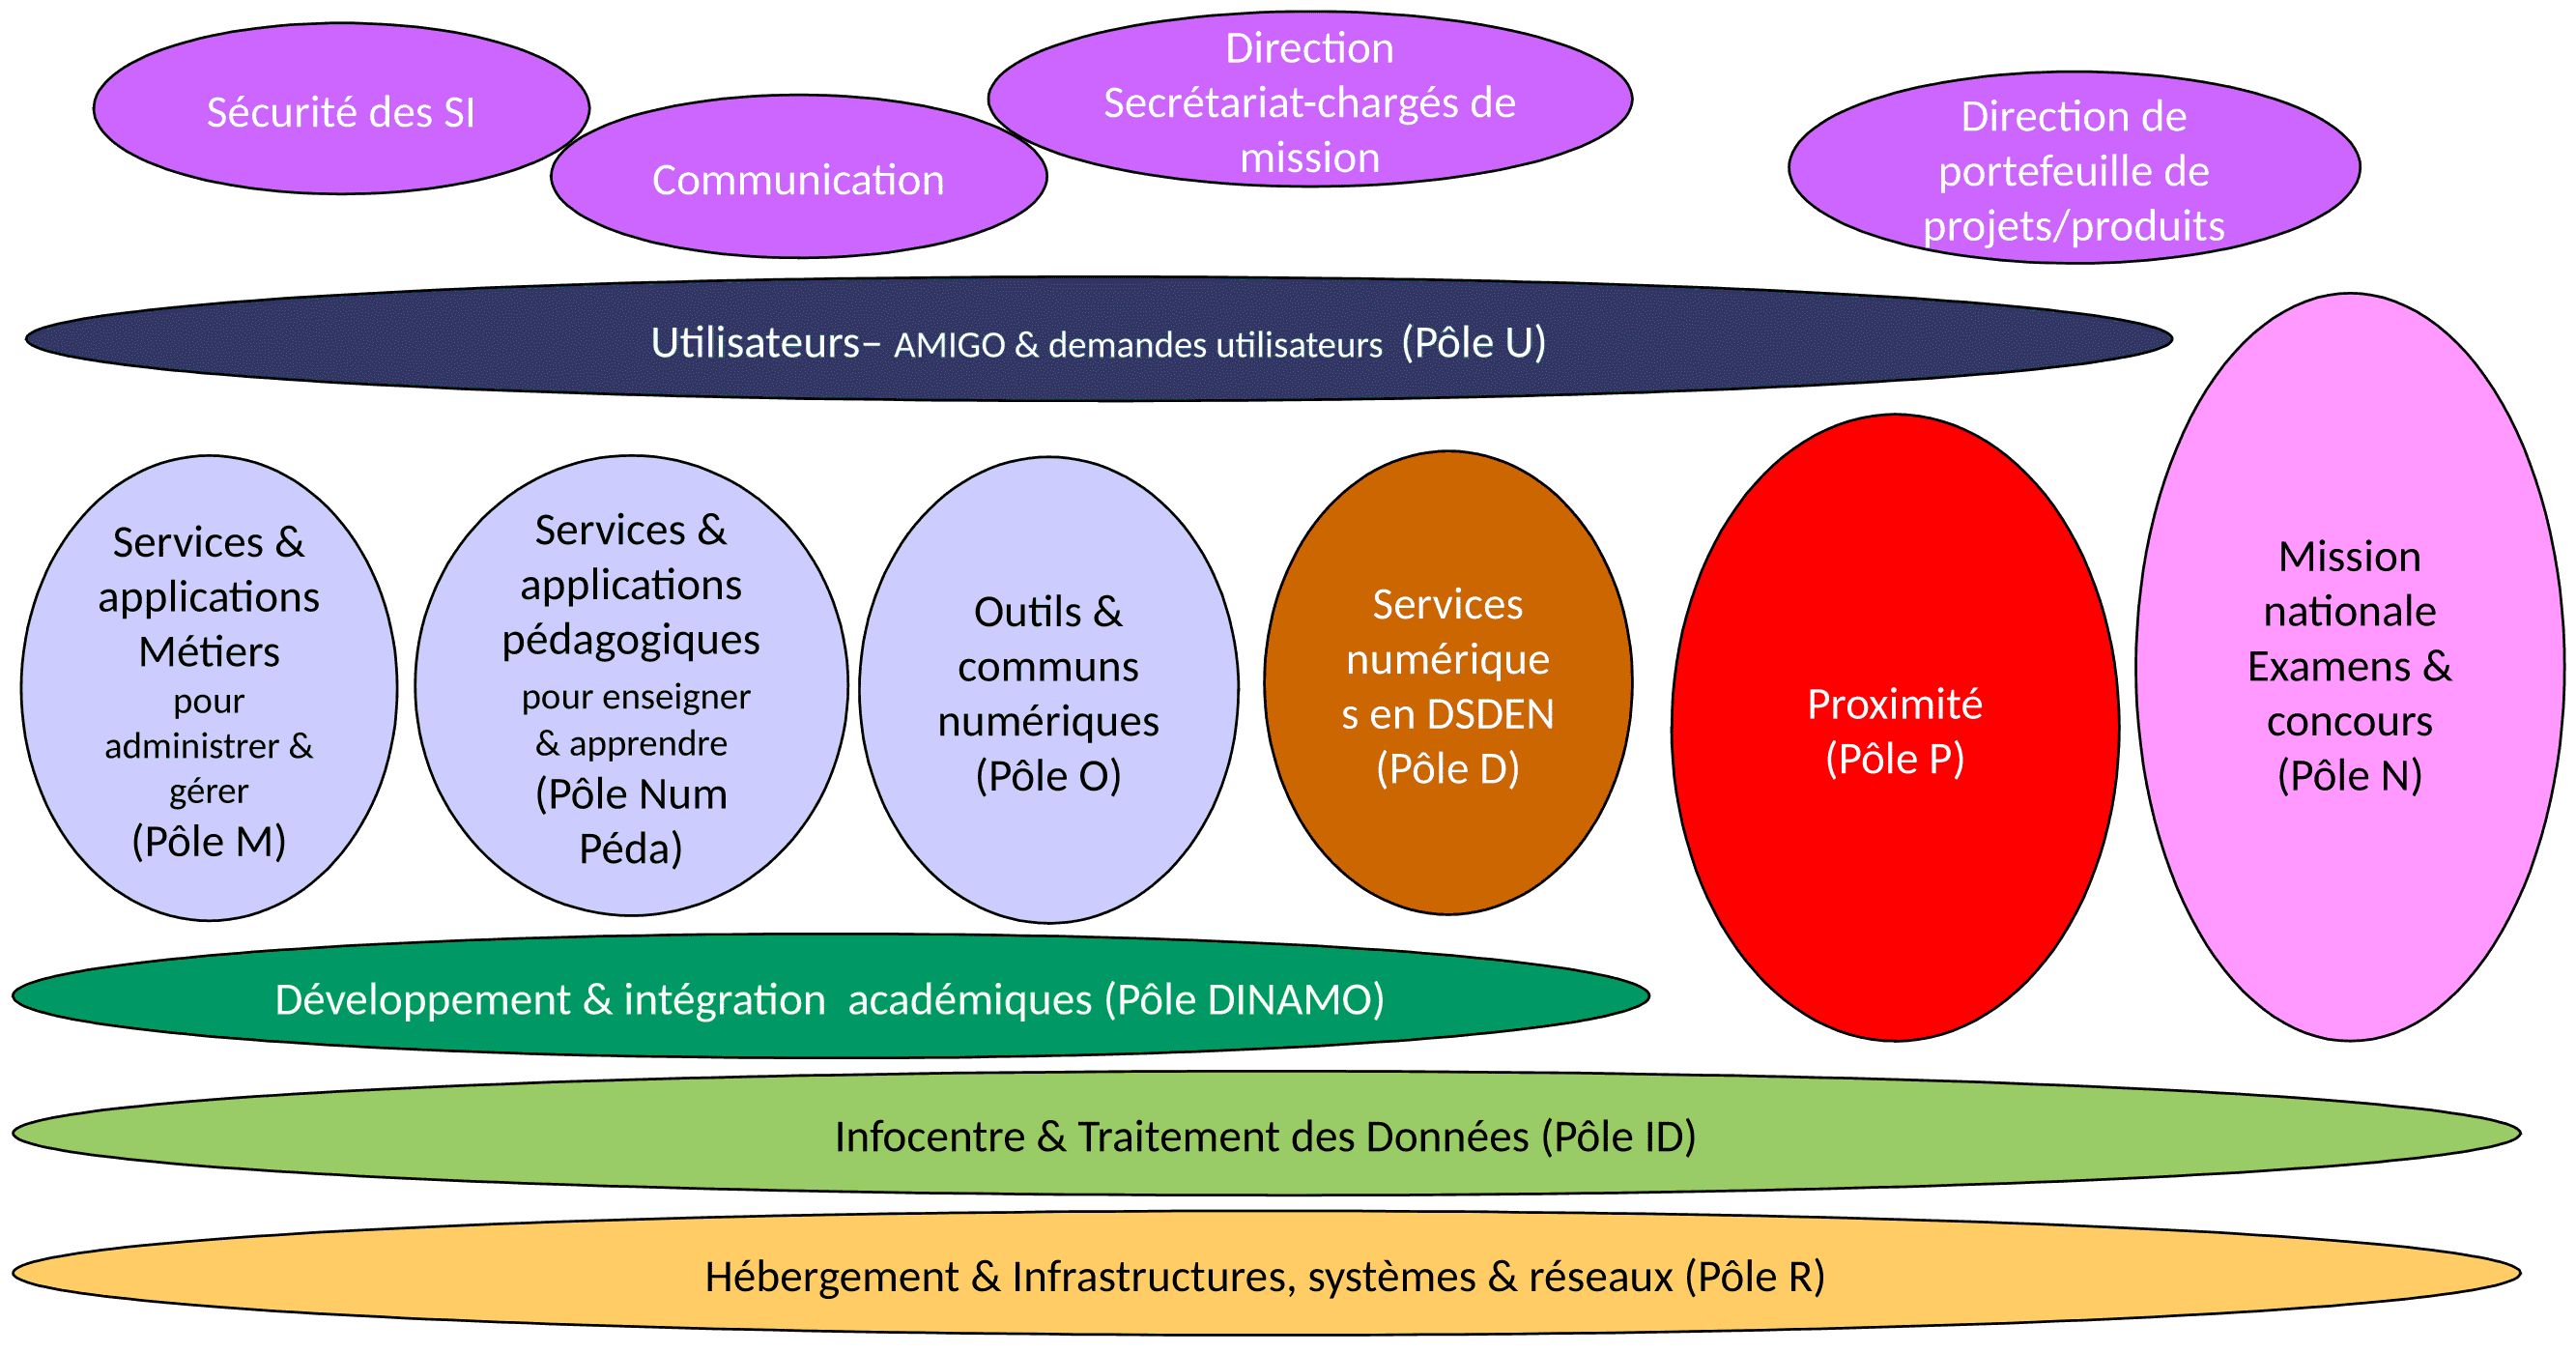
\includegraphics[width=1\textwidth]{diagrammes/organigramme_DSII.png}
  		\caption{Organigramme fonctionnel du service informatique académique}
	\end{figure}

\end{itemize}

\subsection{Pôle DINAMO}

Au sein du rectorat, nous trouvons le pôle DINAMO (Développement et INtégration en environnement Académique ou Mutualisé), dans lequel je travaille en tant qu'apprenti et dont l'activité principale est le développement et l'intégration académiques. 


\begin{enumerate}
\item \textbf{Missions :}\\

\begin{itemize}
\item  Mettre en œuvre des services numériques académiques ou mutualisés.
\item  Réaliser des applications web et fournir des applications fiables, sécurisées et adaptées aux usages des utilisateurs. 
\item  Assurer la maintenance et l'évolution des projets.\\
\end{itemize}

\item \textbf{Effectifs :}\\
L’équipe de développement du pôle DINAMO est constituée d’Arnaud Rupin, responsable du pôle, ainsi que 6 développeurs informatiques (Albane GUIHOMAT, Annabel BOURDÉ, Gaël SALAÜN, Maïna DIRINGER, Marc BERHAUT et Vincent CARON). Voir figure 2\\

\end{enumerate}

\begin{figure}[H]
	\centering
 		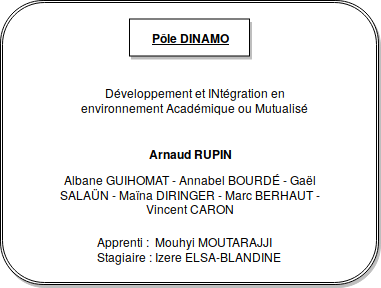
\includegraphics[width=1\textwidth]{diagrammes/PoleDinamo.png}
  		\caption{l'équipe du pôle DINAMO}
	\end{figure}


\subsection{Méthodes de travail}
\subsubsection{Méthodologie agile}

Les projets de l'équipe DINAMO fonctionnent en méthodologie agile sous forme de sprints qui varient de 2 à 4 semaines. Chaque équipe effectue un Daily-meeting afin d'échanger sur l'évolution des tâches à faire.

Durant un sprint, l'équipe embarque des nouvelles \textbf{User Story}\footnotemark et réalise des nouvelles fonctionnalités ou corrige les erreurs et les bugs rencontrés lors des démos. Le lancement de chaque sprint se fait lors d'une réunion \textbf{sprint planning} dans laquelle toute l'équipe du projet est présente ainsi que le PO, ce dernier désigne les nouvelles \textbf{User Story} et les nouvelles fonctionnalités qu'il souhaite voir rajoutées ou corrigées dans la prochaine version de l'application. Le client est présent lors de la démo pour vsualiser l'avancement du projet ou suggérer des corrections. 
\footnotetext{Un récit utilisateur, ou « user story »  en anglais, est une description simple d’un besoin ou d’une attente exprimée par un utilisateur et utilisée dans le domaine du développement de logiciels et de la conception de nouveaux produits pour déterminer les fonctionnalités à développer.}.

Durant mon alternance, j'ai eu la chance d'être invité par mes maîtres d'alternance à assister à plusieurs réunions d'autres projets afin de voir le déroulement d'un projet agile. J'ai pu assister à un sprint planning, une rétrospective , une démo, etc...    

Dans mon cas, j'étais le seul développeur dans mon projet, je faisais un Daily-meeting avec mes maîtres d'alternance pour que je puisse dire sur quoi je travaillais et leurs poser des questions en cas de blocages. L'administrateur des systèmes d'informations(ADSI) Clément JOSSO, qui est en même temps le Product Owner(PO) du projet, et mes maîtres d'alternances me conseillaient sur l'ordre des tâches à suivre lors des multiples réunions.   

\subsubsection{Communication}

Pour communiquer, l'équipe informatique utilise l'outil de messagerie instantanée Rocket.Chat. Il permet de créer différents
channels pour chaque équipe, des channels de veille ont été également crées pour de la veille technologique.

Nous utilisons aussi l'outil Calendar (un outil développé par Oracle) qui permet d’organiser les réunions.  

\subsubsection{Dockerisation}

Le logiciel Docker permet de créer, déployer et exécuter des conteneurs de manière efficace. Un conteneur enveloppe l’application d’un logiciel dans une boîte invisible avec tout ce dont il a besoin pour s’exécuter.


Dans le pôle DINAMO, l'équipe utilise Docker Compose pour partager le même environnement de travail entre plusieurs personnes et tout installer sur docker. Docker Compose est un outil qui permet de décrire et gérer  plusieurs conteneurs comme un ensemble des services inter-connectés.

Dans les projets sur lesquels j'ai travaillés, nous avons utilisé Docker Compose pour déclarer tous les conteneurs dont nous avons besoin dans un fichier .yml  et nous démarrons l'ensemble des conteneurs en une seule commande \textbf{docker-compose up}. 

Dans le fichier docker-compose.yml, chaque conteneur est décrit avec un ensemble de paramètres qui correspondent aux options disponibles lors d’un docker run : l’image à utiliser, les volumes à monter, les ports à ouvrir...
 

\subsubsection{Versionning}

L'équipe informatique utilise Git sur la plateforme Gitlab hébergée par la Forge Nationale comme gestionnaire de versions. 

\section{À propos du projet}

\subsection{Contexte et Problématique}

La DSII (Direction des Systèmes d'Information et d'Innovation) et plus précisément l'équipe DINAMO utilise plusieurs façons pour documenter leur applications. La plupart du temps elle utilise une documentation écrite (Manuel Utilisateur). Cette documentation est souvent pas lu à cause de contrainte de temps, ce qui rend difficile aux utilisateurs de se documenter sur l'applcation.


C'est pour cette raison que Monsieur JOSSO Clément,le product Owner du projet(PO), a voulu mettre en œuvre une documentation interactive dans l'application métier Solycee afin de faciliter l’accès de la documentation à ces utilisateurs et d'interagir directement avec l'application via une interface graphique. Nous avons utilisé un outil nommé BootstrapTour pour réaliser cette documentation. 

Le besoin du client est d'avoir une application qui permet à l'ADSI(Administrateur Des Systèmes d'Informations) de créer la documentation directement à partir de sa page web et pouvoir l'améliorer au fur et à mesure des demandes des utilisateurs via une interface graphique rajoutée dans le projet Solycee. 


Le but final du projet est de permettre aux ADSI d'être autonomes et de pouvoir rajouter la documentation dans leurs applications. Nous avons implémenté un web service(AppTour) qui permettra aux ADSI de rajouter la documentation et la sauvegarder, nous avons donc ajouté une interface graphique dans l'applciation Solycee pour faire appel au web service AppTour.
 
\subsection{Présentation de Bootstrap Tour : Une visite guidée interactive}
 
Bootstrap Tour est une librairie JavaScript permettant de présenter de façon assez simple l’application. Bootstrap Tour est une implémentation qui sert à créer une visite guidée pour une application.

Le bénéfice de l'utilisation de Bootstrap Tour est immédiat pour les utilisateurs car elle présente les fonctionnalités de la page directement sur l'écran soit en lançant la documentation  dès l'ouverture de la page ou en appuyant sur un bouton pour déclencher cette documentation.\\
\textbf{Mise en œuvre et  Utilisation :}

Pour utiliser une visite guidée par Bootstrap Tour, il faut récupérer les bibliothèques et les sources dont nous avons besoin. La première étape est de construire un "Tour" qui accepte un bon nombre de paramètres dont le paramètre "Step" (étape). Ensuite il suffit de donner des étapes à notre tour, pour chaque étape il faut définir certains attributs : 

\begin{itemize}
\item \textbf{Élement: } Élément sur lequel vous désirez afficher votre popup. une popup est une fenêtre modale apparaît au-dessus de la page et est en général utilisée comme une boîte de dialogue avec l’utilisateur. 
\item \textbf{Title: } Titre affiché sur la popup. 
\item \textbf{Content: } Message affiché dans le corps du popup.
\item \textbf{placement: } Permet d’indiquer dans quel sens vous désirez afficher la popup.
\end{itemize} 



\subsection{Architecture du projet}

Le projet se constitue de rajouter une interface utilisateur sur l'application web (Solycee) et  implémenter une API REST (AppTour) qui communique avec une base de données relationnelles. Voir figure 3.

\begin{enumerate}
\item \textbf{Technologies :}\\

\begin{itemize}
\item \textbf{Java: }Langage du développement du Back-end de Solycee. 
\item \textbf{Kotlin: }Langage du développement de l'API Rest AppTour. 
\item \textbf{Maven: }Construction des projets Java et Kotlin du Back-end.
\item \textbf{Spring: } Framework du développement du Back-end de Solycee.
\item \textbf{JavaScript,CSS,HTML,Bootstrap: } Développement du Front-end de Solycee.
\item \textbf{JUnit: } Framework de test des Back-end Solycee et AppTour. 
\end{itemize} 
\end{enumerate}

\begin{figure}[H]
	\centering
 		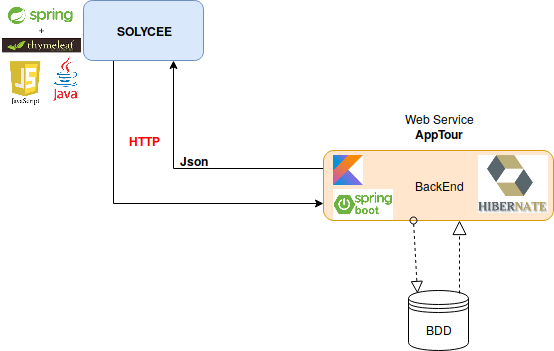
\includegraphics[width=1\textwidth]{diagrammes/ArchitectureGenerale.png}
  		\caption{Architecture du projet}
	\end{figure}\\

Nous avons une application web nommée Solycee qui communqiue avec une API REST nommée AppTour via des requêtes HTTP(CRUD), ces dernières renvoient des réponses en format Json. 

\section{Objectifs et missions de l'alternance}

\subsection{Solycee}

Solycee est une application métier créée par le pôle DINAMO et destinée à la gestion des offres et demandes de stages de découverte. Elle permet aux collèges et aux lycées d'inscrire leurs élèves dans des mini-stages proposés par les lycées.  

 
\subsubsection{Architecture de l'application Solycee}

\begin{figure}[H]
    \centering
    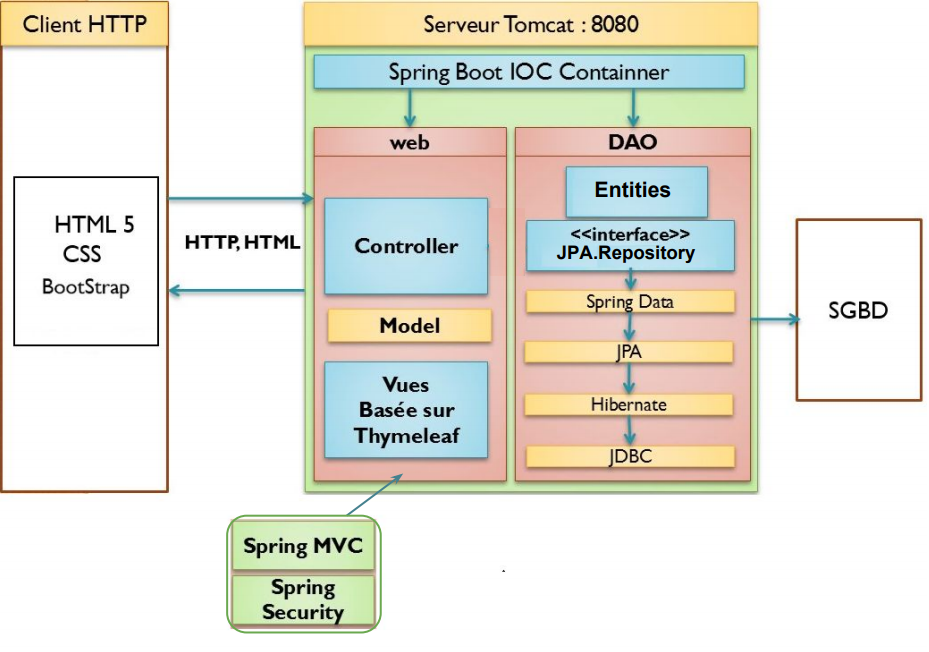
\includegraphics[width=0.9 \textwidth]{diagrammes/archiSolycee.png}
    \caption{Architecture logicielle de l'application Solycee }
\end{figure}

\subsubsection{Aspect technique}

Le projet est implémenté selon le patron de conception MVC et réalisé avec plusieurs technologies, la plupart de ces dernières sont open-source.L'application est implémentée avec un Back-end et un Front-end.

Le Back-end est réalisée en Java avec l'utilisation des composants du framework Spring.L'interface est codée avec le triplet HTML,CSS \& Javascript, les vues sont basées sur Thymeleaf. 

Voici maintenant une présentation plus précise sur les principaux outils utilisés:\newline

\textbf{Spring:} Spring est un framework libre pour construire et définir l'infrastructure d'une application java dont il facilite le développement et les tests. Le concept fondamental de Spring, qui fait sa force, est l'injection des dépendances (dependency injection).\newline

\begin{itemize}
	\item \textbf{Spring MVC} : Spring MVC est un framework qui permet d’implémenter des applications selon le design pattern MVC. Spring MVC se base sur le principe décrit par le schéma ci-dessous :\newline
	

\begin{figure}[H]
	\centering
 		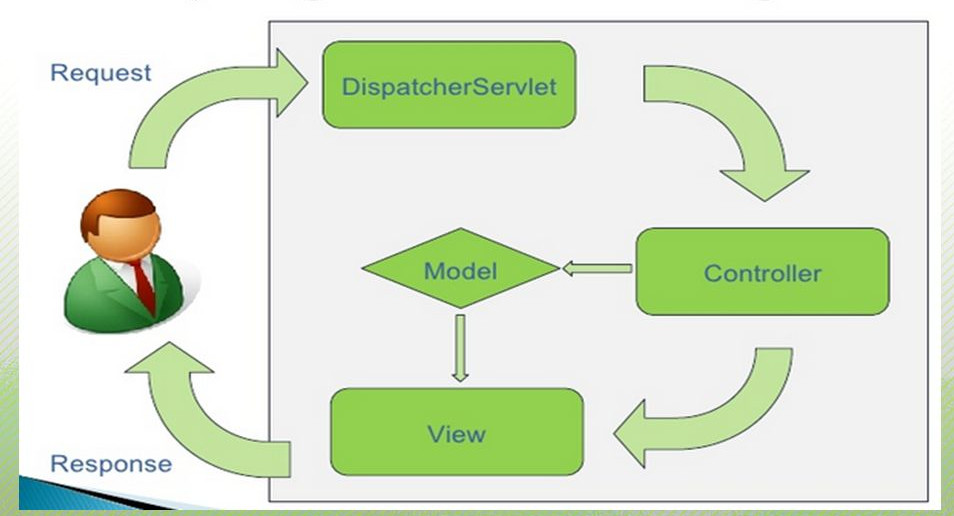
\includegraphics[width=1\textwidth]{diagrammes/mvc2.jpg} 
  		\caption{Schéma du patron de conception MVC}
	\end{figure}
	
	Spring MVC s'appuie sur :

    - une servlet principale appelée Dispatcher Servlet qui va gérer l'intégralité 			  des requêtes HTTP reçues.\\
    - un handler mapping qui va faire le lien entre l'URI appelée et le contrôleur    	  MVC.\\
    - le Controller qui va gérer le rôle du contrôleur MVC et qui va solliciter le 			  modèle.\\
    - View Resolver qui va préparer la vue en fonction du code retour du Controller
      la View qui assure le rôle de vue au sens MVC.

	
	\item \textbf{Spring Security }: Spring Security est un Framework de sécurité  qui fournit une authentification et un support d’autorisation afin de sécuriser les applications Spring. \newline
\end{itemize} 

\textbf{Maven:} Maven est un outil de construction de projets (build) open source développé par la fondation Apache. Il permet de faciliter et d'automatiser certaines tâches de la gestion d'un projet Java. Le but est de produire un logiciel à partir de code source en optimisant les tâches à réaliser. Il est facile à configurer.\newline

\textbf{Hibernate: } Hibernate est un framework open source de type ORM (Object Relational Mapping) qui permet de faciliter le développement de la couche persistance d'une application. Il permet donc de représenter une base de données en objets Java et vice versa.

\textbf{Thymeleaf:} Thymeleaf est un Java XML/XHTML/HTML5 moteur de templating qui apporte le concept de templates en utilisant des attributs HTML spécifiques. Ce framework apporte aussi une séparation entre l'affichage et le contenu.\\

Thymeleaf s’intègre très facilement dans un projet Spring et permet de diffuser XHTML/HTML5 sur la vue des applications WEB.


\subsubsection{Travail réalisé}


Dans le projet Solycee, j'ai principalement travaillé sur la partie Front-end. J'ai réalisé plusieurs tâches soit en rajoutant des nouvelles vues et des nouveaux composants dans les pages web et/ou en rajoutant des nouvelles fonctionnalités sur les composants existants.

Le projet a été développé par l'équipe Dinamo. Avant de commencer à réaliser les tâches demandées, il était nécessaire de procéder un travail  de lecture du code implémenté et de la compréhension de ce dernier en posant des multiples questions à mes maîtres d'alternances. Il m'a fallu aussi comprendre l'architecture du projet ainsi que les technologies utilisées. 

Une fois que le code était compris et que j'ai acquis toutes les informations importantes sur le projet, j'ai commencé à réaliser les tâches demandées.

J'ai commencé par manipuler Bootstrap Tour sur l'application Solycee en intégrant le code de la librairie dans le front-end de Solycee (code en javascript avec les étapes souhaités). Suite à une demande de l'ADSI de Solycee nous avons pu réaliser une première version(V1) en utilisant Bootstrap Tour. Un tour est défini dans un fichier JavaScript et il est composé de différentes étapes. Bootstrap Tour permet d'afficher l'étape du tour et aussi passer à l'étape suivante ou précédente ainsi que arrêter le tour avec le bouton "Fin"(Voir Figure 6). Pour lancer la documentation, il faut exécuter deux méthodes dans le fichier Javascript, init et start. 
\begin{figure}[H]
	\centering
 		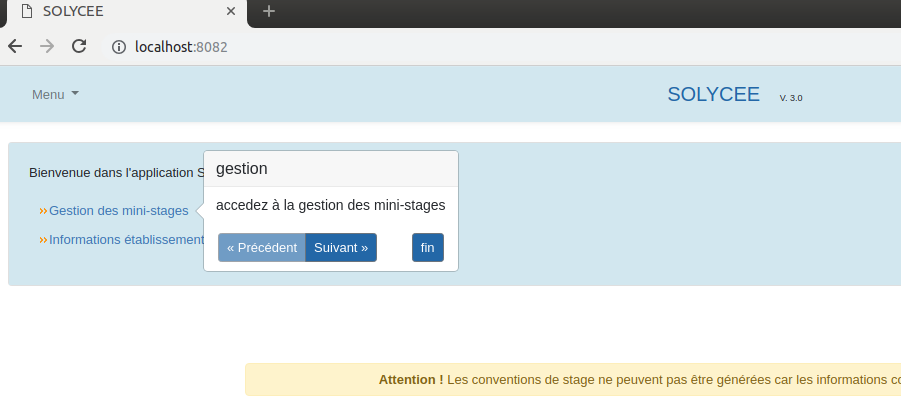
\includegraphics[width=1\textwidth]{diagrammes/exemple_Tour.png} 
  		\caption{Exemple d'une étape de Bootstrap Tour}
	\end{figure}

\begin{enumerate}
\item \textbf{V2: Création de la base de données: }\\

Après avoir livrer une première version au PO, il s'agit de déclancher la documentation via un fichier javasript et suite à une demande du PO, nous avons commencé à travailler sur la deuxième version(V2). Il s'agit de stocker la documentation dans une base de données distante. 

Voici une présentation plus précise des fonctionnalités ajoutés pour la V2 :

\begin{itemize}
\item  L'ajout d'une fenêtre modale pour prévenir les utilisateurs de la présence d'un bouton aide pour déclencher la documentation interactive.Voir Figure 7

\begin{figure}[H]
	\centering
 		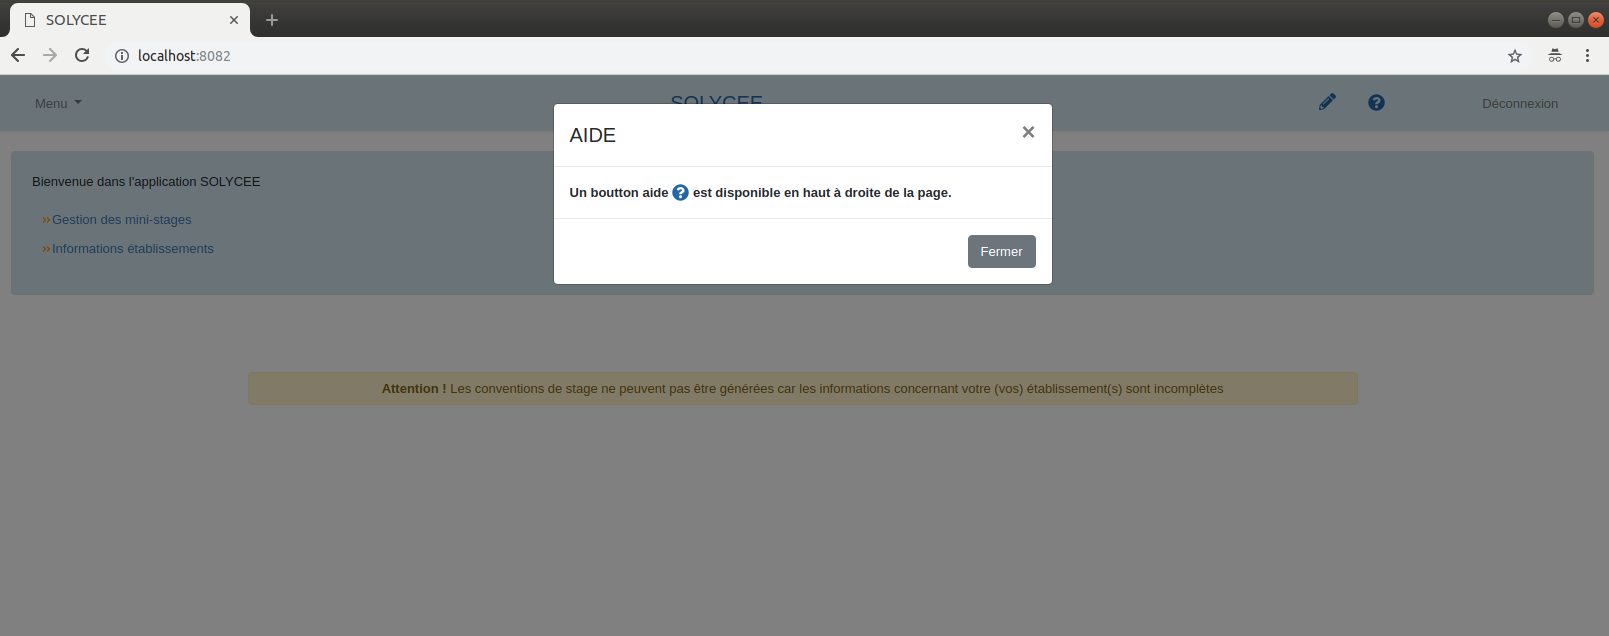
\includegraphics[width=1\textwidth]{diagrammes/aide_modal.png}
  		\caption{Page d'accueil Solycee}
	\end{figure}
Cette modale n'apparaît qu'une seule fois chez les utilisateurs. Elle ne s'affiche que si l'utilisateur consulte l'application Solycee pour la première fois. \\ 


\underline{Mise en oeuvre} :
Pour réaliser cette tâche, j'ai dû ajouter une modale qui est un composant Bootstrap qui s'affiche à la première connexion de l'utilisateur à l'application. Cette modale n'apparaît pas une deuxième fois. \\ 

   
\item  Déclencher la documentation interactive en appuyant sur un bouton: Dans la première version, la documentation se déclenchait dés que l'utilisateur arrive sur la page de l'application et cela peut être répétitif pour l'utilisateur. Dans le cas présent, la documentation s'exécute seulement en cliquant sur un bouton. \\ 

\underline{Mise en oeuvre} :
Rajout du Bootstrap Tour : Il s'agit de l'ajout d'un bouton 
\includegraphics[width=5mm,scale=0.5]{diagrammes/Bouton_aideDispo.png} dans le fichier Decorator, ce fichier est l'entête de toute les vues de l'application Solycee. Il s'agit d'un fichier HTML qui contient le nom de l'application ainsi les composants utilisés par toutes les pages web de Solycee. En appuyant sur le bouton 
\includegraphics[width=5mm,scale=0.5]{diagrammes/Bouton_aideDispo.png} ça déclenche les pop-ups  de Bootstrap tour. 



La mis en place de Bootstrap Tour dans un ficher Javascript était une façon simple pour lancer une documentation interactive. Il faut ajouter des Tours et des Steps dans le fichier JS, donc il faut aller chercher et modifier dans le code, une manipulation qui peut être compliqué des fois et qui ne permet pas aux ADSI d'être autonome et rajouter la documentation souhaitée eux mêmes. 

Nous avons donc créé un web service AppTour où sont sauvegardés les Tours et les Steps. L'application Solycee communique avec ce web service pour récupérer les informations et la documentation. \\ 

\item  Récupérer la documentation d'une page web de l'application Solycee: Il faut faire un appel au Web service AppTour. \\   
 
\underline{Mise en oeuvre} :
- Chaque page HTML(Vue) de l'application Solycee a un identifiant qui correspond à l'Id de son corps "Body".

- Un fichier JavaScript "tourLoader" est importé dans toutes les vues de Solycee.

- Nous interrogeons le Web service AppTour avec une requête Ajax en passant en paramètre le nom de l'application et l'identifiant de la page courante. La requête vérifie s'il existe de la documentation pour l’identifiant concerné. 

- Si la requête renvoie un fichier json qui contient les tours et les étapes à déclencher avec Bootstrap Tour, l'utilisateur peut exécuter une documentation interactive en cliquant sur le bouton 
\includegraphics[width=5mm,scale=0.5]{diagrammes/Bouton_aideDispo.png}. Voir Figure 6.    

- Dans le cas où il n'existe pas de documentation sur la page web, le bouton affiché est gris et titré par une phrase "Aide non disponible pour cette page". Voir Figure 8 \\
\begin{figure}[H]
	\centering
 		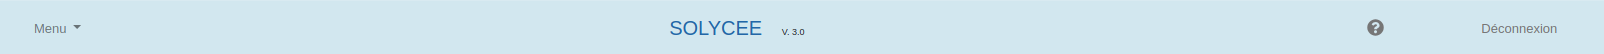
\includegraphics[width=1\textwidth]{diagrammes/aideNonDispo.png} 
  		\caption{Pas de tour disponible dans cette page Web }
	\end{figure}
   

\item \textbf{V3: Séléction des composants et l'ajout de la documentation}\\ 

Après avoir fini la V2 et que l'ADSI pouvait déclancher la documentation à l'aide d'un bouton, nous avons travaillé sur la V3. Il s'agit d'ajouter un mode édition dans l'application Solycee. 

Voici une présentation plus précise des fonctionnalités ajoutés pour la V3:
 
\item  Ajouter un mode d'édition pour les ADSI: Jusqu'à maintenant, les ADSI ne pouvaient pas rajouter la documentation sauf s'ils rajoutent des données en dur dans la base de données. Pour cela, nous avons créé un mode édition dans l'application Solycee qui est présenté par une interface graphique et elle  permet de rajouter la documentation.\\


\underline{Mise en oeuvre} : \\
- Nous avons ajouté le bouton
\includegraphics[width=5mm,scale=0.5]{diagrammes/Bouton_modeEdition.png} dans toutes les pages web de l'application Solycee qui est titré par une  phrase "Veuillez cliquer ici pour passer en mode édition".

- En appuyant sur le bouton 
\includegraphics[width=5mm,scale=0.5]{diagrammes/Bouton_modeEdition.png} les ADSI passent en mode édition pour rajouter la documentation souhaitée sur n'importe quel composant de la page web.Nous affichons un champs sur l'interface pour prévenir les ADSI qu'ils sont passés en mode édition.Voir Figure 9.

\begin{figure}[H]
	\centering
 		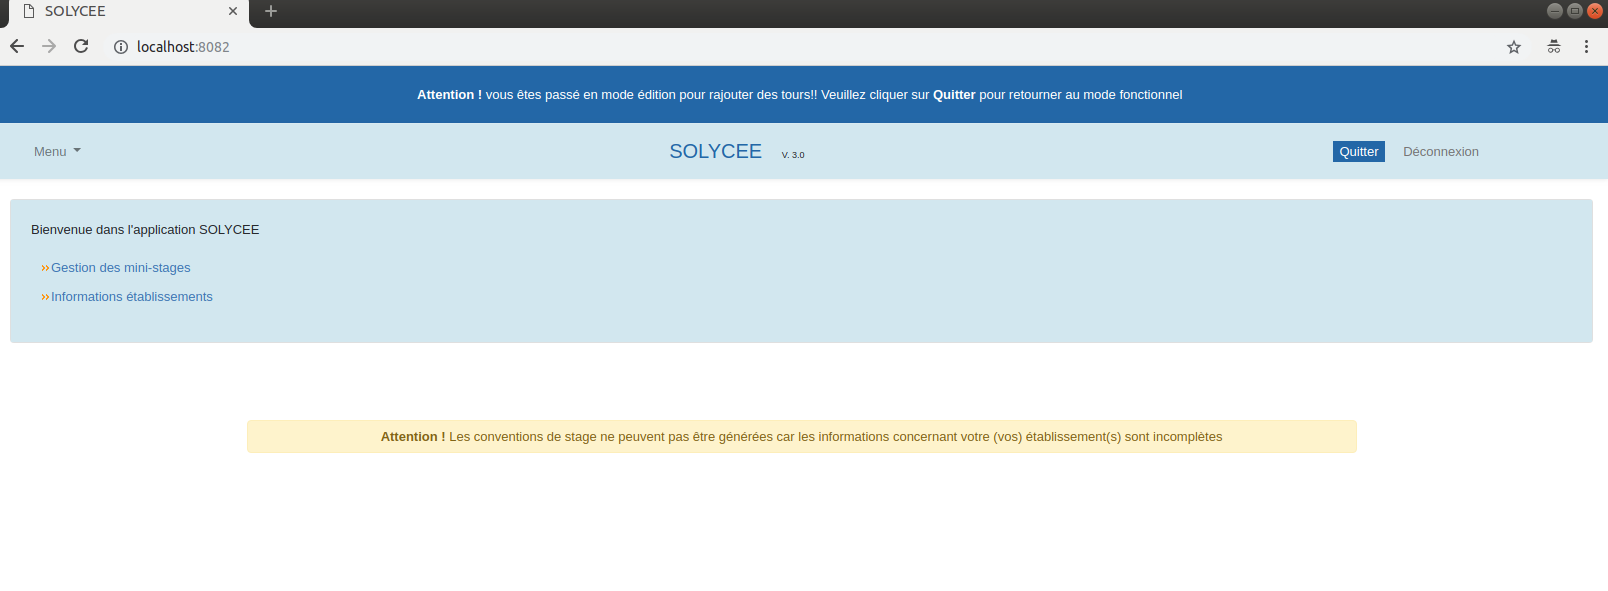
\includegraphics[width=1\textwidth]{diagrammes/mode_edition.png} 
  		\caption{Page d'accueil en mode édition}
	\end{figure}
 
Ce mode consite à désactiver le fonctionnement de tous les composants de la page web(boutons, url,logo,etc...), par exemple si l'utilisateur appuie sur une url, la page web ne se dirige plus vers l'url. Par contre, Si l'ADSI appuie sur un composant de la page alors qu'il est en mode édition, cela affiche une modale qui contient plusieurs champs(Titre,Élément,Contenu...) créés en HTML et CSS.

\begin{itemize}
\item \textbf{Élement: } Id de l'élément sélectionné. 
\item \textbf{Title: } Titre affiché sur la popup. 
\item \textbf{Content: } Message affiché pour expliquer le fonctionnement du composant appuyé.  
\end{itemize}


\item  Remplir les champs de la modale : Quand les ADSI passent en mode édition et en appuyant sur un composant de la page web, la modale s'affiche qui permet de rajouter ou modifier la documentation. Ensuite, nous remplissons les champs de la modale dans le cas où il existe une documentation pour ce composant. \\

\underline{Mise en oeuvre} : 

- En appuyant sur un composant de la page, nous envoyons une requête HTTP en utilisant Ajax au Web service AppTour pour récupérer l'étape dans le cas où elle existe. Nous passons en paramètre l'identifiant de l'élément appuyé ainsi que l'id du tour de la page web où se trouve l'ADSI. 

- Si l'étape existe dans la table Step de AppTour, nous récupérons l'objet et puis nous remplissons les champs par les données récupérées(Title \& content).Voir Figure 10.

\begin{figure}[H]
	\centering
 		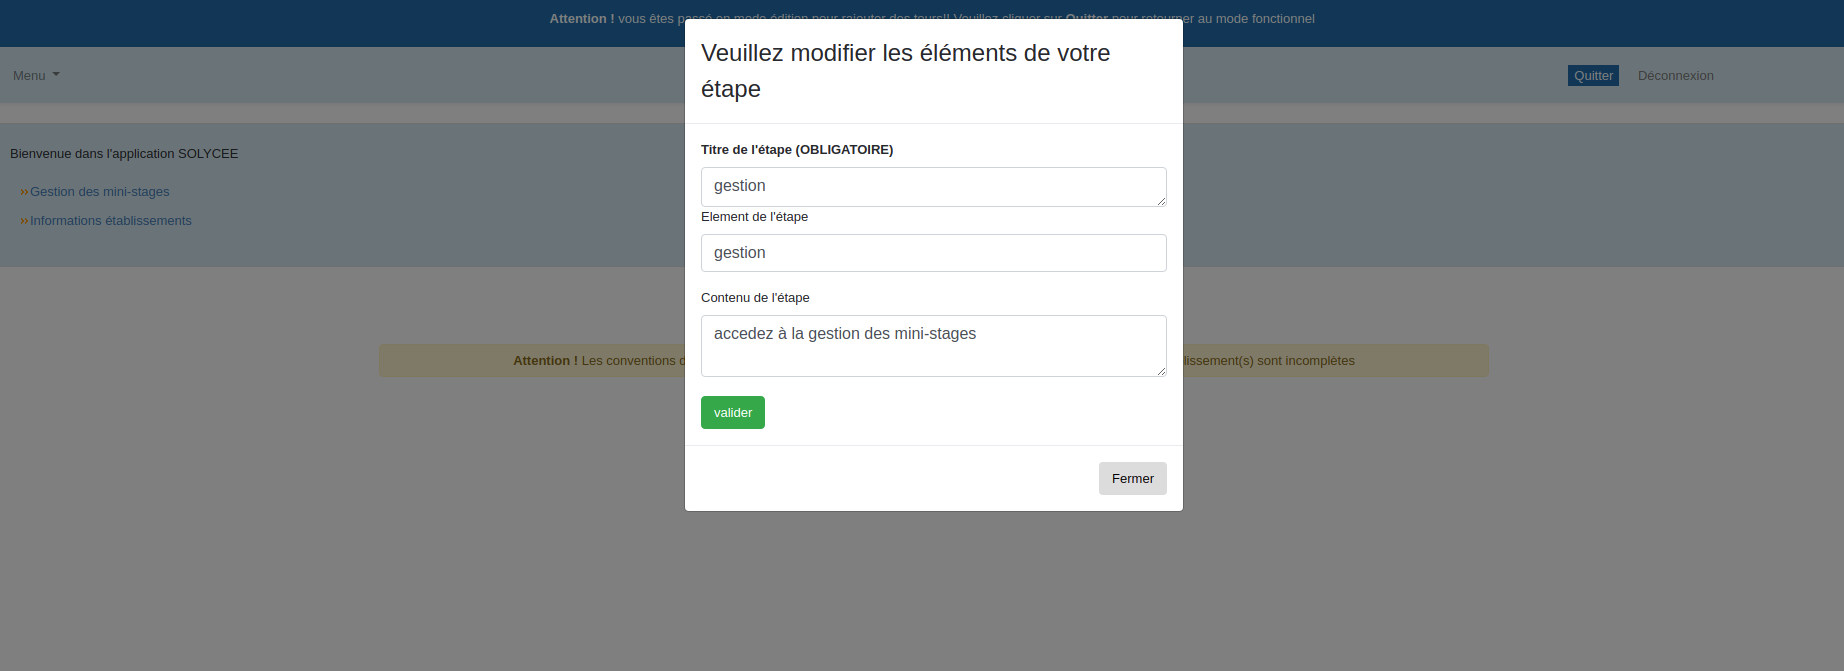
\includegraphics[width=1\textwidth]{diagrammes/Modal_gestion.png} 
  		\caption{une documentation existe déjà pour le lien Gestion des mini-stages}
	\end{figure}

- Dans le cas où il n’existe pas de documentation pour l'élément sélectionné, nous laissons les champs vides.\\ Voir Figure 11.

\begin{figure}[H]
	\centering
 		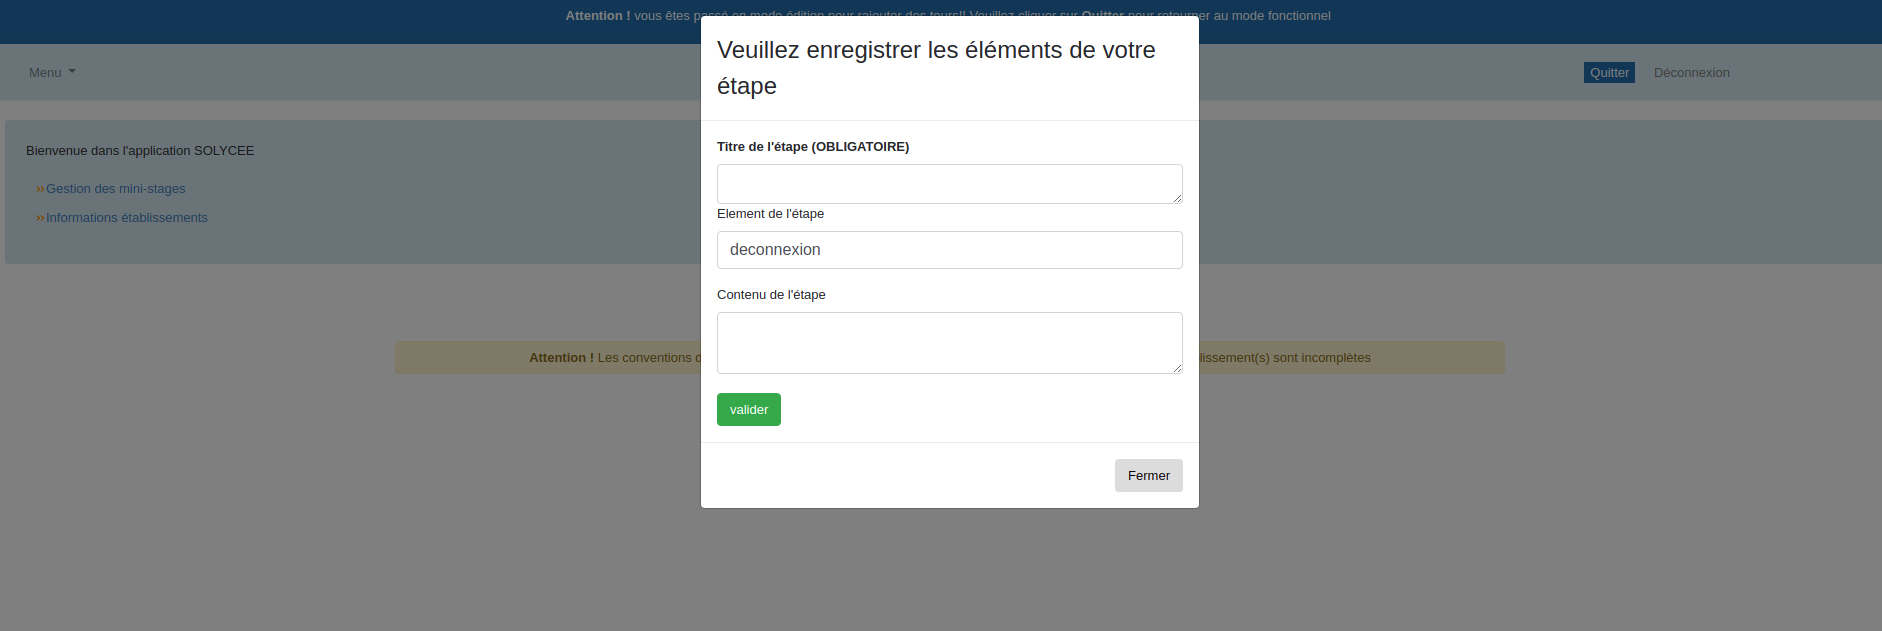
\includegraphics[width=1\textwidth]{diagrammes/Modal_Deconnexion.png} 
  		\caption{Pas de documentation pour le bouton Déconnexion}
	\end{figure}

\item Ajouter ou modifier la documentation : Quand l'ADSI est en mode édition, il peut soit ajouter la documentation pour un composant de la page web dans le cas où il n'existe pas de documentation pour ce dernier, soit la modifier dans le cas où elle existe. 
 
\underline{Mise en oeuvre} : 

- Après que nous interrogeons le Web service AppTour sur la présence de la documentation pour le composant appuyé, si elle est présente nous remplissons les champs et l'ADSI peut la modifer en changeant le contenu de l'étape ou son titre. Le bouton valider de la modale permettra alors d'envoyer une requête Ajax (PUT) au Web service pour stocker les  modifications faites sur l'étape. 

- Dans le cas où il n'existe pas de documentation pour l'élément appuyé, l'ADSI peut remplir les champs vides(Mettre un titre à la nouvelle étape et un contenu pour expliquer le fonctionnement de l'élément). Le bouton valider permet cette fois d'envoyer une requête Ajax (POST) pour rajouter la nouvelle étape dans la table Step.  

\end{itemize}

\end{enumerate}

\subsection{AppTour}   

Comme expliqué plus haut, au début nous avons commencé par manipuler Bootstrap Tour en écrivant du code et en utilisant la librairie JS(Bootstrap Tour). Pour cette raison, nous avons créé le Web service AppTour afin de permettre aux ADSI des applications d'être autonome et pouvoir rajouter la documentation interactive tout simplement en interrogeant le web service. Ils peuvent rajouter des étapes à des tours existants ou même rajouter des nouveaux tours.Nous avons donc implémenté plusieurs Endpoint afin d'exposer leurs documentations.  
 
\subsubsection{Architecture de l'API AppTour}

Le Back-end AppTour, c’est la partie du code qui est exécutée par le serveur, il s'agit d'une API Rest qui gère la persistance des données et la logique de l'application. 
 

Le Back-end Apptour se compose de plusieurs couches: \newline

- Une couche Model: Cette couche représente le modèle de données objet de l'application. \newline

- Une couche Repository/DAO: Repositories sont des interfaces héritant de l'interface Repository. L'objectif de ces interfaces consiste à rendre la création de la couche d'accès aux données (requêtes SELECT, UPDATE...) plus simple. Cette couche s'appuie sur l'interface JPA (Java Persistence API) qui permet la persistance des données.\newline


- Une couche Service: Cette couche implémente l'ensemble de la logique métier de l'application. Elle s'appuie sur les couches DAO et model pour effectuer des opérations CRUD (Create, Read, Update, Delete) sur des objets persistés et leur appliquer ensuite des traitements métier.\newline


- Une couche Controller: Il s'agit de l'API qui permet de répondre à toutes les requêtes envoyées par le client. 



\begin{figure}[H]
	\centering
 		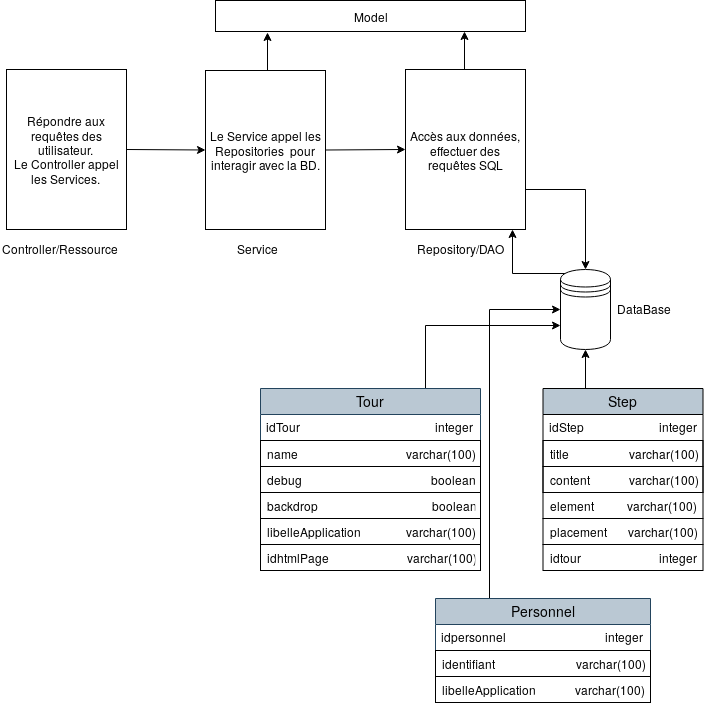
\includegraphics[width=1\textwidth]{diagrammes/Architecture_Apptour.png}
  		\caption{Architecture Back-end d'une application web}
	\end{figure}
	

Voici le cycle  d'appel de l'application Solycee au web Service Apptour:  

\begin{figure}[H]
	\centering
 		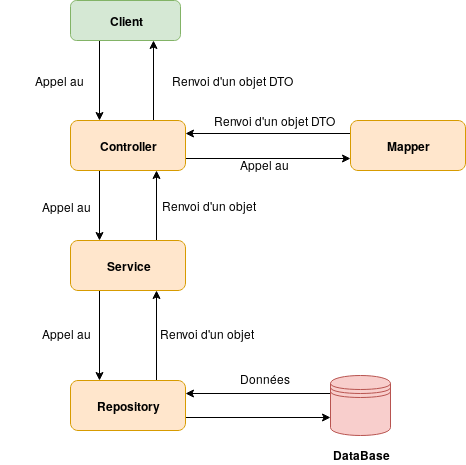
\includegraphics[width=1\textwidth]{diagrammes/schema_apptour.png}
  		\caption{Cycle d'une interrogation au web service}
	\end{figure}

\subsubsection{Aspect technique}

L'API Rest AppTour est une application Spring Boot codée en langage Kotlin. Voici une présentation plus précise sur les principaux  
outils utilisés: 
\textbf{Spring boot:} Est un framework utilisé afin de faciliter la configuration d'un projet Spring et de réduire le temps alloué au démarrage d'un projet.

\textbf{Kotlin:} Kotlin est un langage de programmation orienté objet et fonctionnel, il a plusieurs avantages, voici les plus importants :
\begin{itemize}
\item \textbf{Typage statique: } Kotlin est un langage de programmation à typage statique. Cela signifie que le type de chaque variable et expression est connu au moment de la compilation.
\item \textbf{Mutabillité: } TODO..
\item \textbf{Sécurisé: } Kotlin est sécurisé. Il évite les exceptions NullPointerExceptions en prenant en charge la nullabilité dans le cadre de son système de types.
\item \textbf{Facile à apprendre: } La syntaxe ressemble beaucoup à la syntaxe Java.
ect.
\end{itemize} 

- \textbf{JUnit:} Pendant mon développement de l'API AppTour, j'ai utilisé la méthode du TDD(Test Driven Development),le développement piloté par les tests. j'ai utilisé le framework JUnit pour implémenter les tests unitaires afin d'assurer la maintenance et l'efficacité de l’application.

-D'autres technologies déjà expliquées précédemment comme Maven, Hibernate, Git

Nous utilisons aussi quelques technologies pour l'intégration continue qui est un ensemble de pratiques utilisées en génie logiciel consistant à vérifier,à chaque modification de code source, que le résultat des modifications ne produit pas de régression dans l’application développée, voici les outils utilisés pour l'intégration continue: 

\textbf{Gitlab:} 
\includegraphics[width=7mm,scale=0.5]{diagrammes/gitlab.png}

Le dépôt central du code source de l’application est un serveur Gitlab. C’est une plateforme complète avec une interface graphique simple et moderne. Gitlab permet de gérer les branches git et les merge-requests en quelques clics, il simplifie la collaboration des contributeurs du développement de l’application. 

\textbf{Jenkins:}
\includegraphics[width=7mm,scale=0.5]{diagrammes/jenkins.png}

Jenkins est un outil logiciel d’intégration continu. Il s’agit d’un logiciel open source. En utilisant ce logiciel, les développeurs peuvent détecter et résoudre les problèmes dans une base de code et rapidement. Ainsi les tests de nouveaux builds peuvent être automatisés, ce qui permet d’intégrer plus facilement des changements à un projet, de façon continue. L’objectif de Jenkin est en effet d’accélérer le développement de logiciels par le biais de l’automatisation. Jenkins permet l’intégration de toutes les étapes du cycle de développement.


La documentation de Jenkins est très riche, et l’outil est devenu bien populaire grâce à sa communauté immense, dynamique et réactive.\\
\newpage
\textbf{Sonarqube:}
\includegraphics[width=30mm,scale=0.5]{diagrammes/sonarqube.png}

C’est un outil qui permet de faire l’inspection continue du code source dans un processus de CI. Une plateforme open-source avec une interface graphique simple et intuitive. Il peut faire une analyse de plus de vingt langages différents tels que JAVA, JavaScript, PHP...\\
Il permet une analyse automatisée en l’integrant dans d’autres serveurs de CI tels que Jenkins, ou projets Maven, Gradle ou Ant. Il est extrêmement complet en terme de fonctionnalités pour la gestion des analyses dans un processus CI:

• Supervision du respect des règles (prédéfinie par l’utilisateur) de programmation.

• Analyse des designs ou l’architecture.

• Évaluation de la couverture du code par les tests unitaires.

• Détection des bugs et des duplications du codes.
 
\subsubsection{Travail réalisé}

Dans le projet AppTour, j'ai travaillé sur la réalisation d'une API Rest, j'ai développé plusieurs endPoints qui permettent de rajouter ou modifier les étapes des tours ainsi que faire des recherches pour vérifier l’existence des tours. 

Comme noté plus haut, le projet AppTour était initialisé par l'alternant précédent, il a initialisé le projet avec la création des tables Tour et Step. j'ai commencé donc par la relecture du code existant et la modification des tables. Ensuite, Nous avons travaillés avec mes maîtres d'alternance sur l'architecture du projet.

Une fois que le code et le travail demandé étaient compris et acquis, j'ai commencé par implémenter les endPoints nécessaire au projet. Voici une présentation plus précise de toutes les tâches réalisées:   

\begin{itemize}

\item  Ajouter des nouveux attributs dans les tables de la base de données. J'ai ajouté dans l'entité Tour  l'atrribut Storage qui permet de garder l'historique des tours éxecutés ou non en mettant l’attribut Storage à True ou False.
  
J'ai ajouté aussi l'attribut Ordre dans l'entité Step pour donner un ordre  d’exécution des étapes de Bootstrap Tour. 

\item Créer toutes les classes DTO afin de les utiliser dans les requêtes  pour envoyer ou récupérer des données.

\item Créer les classes Repositories en utilisant l'interface JpaRepository qui permettent de faciliter l'accès ou le stockage des données dans la base.

\item Créer des classes Mapper qui permettent de convertir un objet Dto à un objet métier ou l'inverse. Par exemple passer d'un objet TourDto à un objet Tour il suffit d'appeler la méthode tourDtoToTour et qui prend en paramètre un objet tourDto : TourDto.  

\item Réaliser l'API et tous les EndPoints, il s'agit d’implémenter des classes controllers qui consomment toutes les méthodes qui se trouvent dans les classes services. Il existe plusieurs types de EndPoints: 

\underline{Mise en oeuvre} : 
\begin{itemize}
\item Des méthodes GET : Pour la récupération des données de la base dans le cas où elles existent.

\item Des méthodes POST : Pour stocker des nouveaux objets dans la bas de données.

\item Des méthodes PUT : Permettre aux ADSI de modifier la documentation déjà existante. 

\end{itemize}
\item Implémenter des classes Services: Toutes les actions effectuer par le controller doivent passer par les classes services. Les services manipulent les objets métiers.

Il existe une classe TourService: Dans cette classe, j'ai réalisé plusieurs méthodes qui permettent de stocker ou récupérer des Tours de la base données : 
\begin{itemize}
\item Chercher un Tour : Elle permet de récupérer un tour en passant en paramètre nom d'une application et l'identifiant de la page HTMl. 

\item Sauvegarder un Tour dans la base de données : Elle permet à stocker un tour dans la base de données en donnant le nom de l'application et l'Id de la page HTML. 

\item Modifier un Tour : Elle permet de modifier un tour existant dans la base données en donnant des nouvelles valeurs. 
\end{itemize}

Il existe aussi une classe StepService : Dans cette classe, j'ai réalisé plusieurs méthodes qui permettent à stocker ou récupérer des Step de la base données : 
\begin{itemize}

\item  Chercher une étape: Récupérer un Step en passant en paramètre l'élément rechercher et l'identifiant du tour.

\item Sauvegarder une étape : Stocker un Step dans la base de données.

\item Lister tout les step d'un tour par ordre croissant.  


\item J'ai aussi créé une table Personnel pour pouvoir l'alimenter par les ADSI des applications de rectorat. Le but final était de pouvoir identifier si la personne connectée d'une application est un ADSI ou pas afin d'avoir le droit d'accéder au mode édition. 

\end{itemize}
\end{itemize}
\subsection{Partie Sécurité}

\subsubsection{Sécuriser le mode édition}
	
	Avant de faire une démonstration au PO et montrer les nouvelles fonctionnalités, un minimum le mode édition, nous avons fait en sorte que seuls les ADSI peuvent rajouter la documentation et non les utilisateurs et ils sont les seuls à accéder à ce mode.\\   
  
  
\underline{Mise en oeuvre} : \\
- Quand l'utilisateur se connecte sur l'application, nous récupérons son identifiant complet.

- Nous interrogeons ensuite le Web service AppTour en utilisant  Srping-RestTemplate\footnotemark, nous envoyons une requête HTTP en passant en paramètre le nom complet d'utilisateur et le libellé de l'application. Si l'utilisateur est présent dans la table Personnel de AppTour, il est ADSI et dans ce cas il a le droit d'accéder au mode édition. Dans le cas inverse, l'utilisateur n'a pas le droit à ce mode et le bouton 
\includegraphics[width=5mm,scale=0.5]{diagrammes/Bouton_modeEdition.png} ne s'affiche pas.
\footnotetext{Spring RestTemplate est une class de Spring qui permet d'établir une communication entre un client et un serveur REST, ceci grâce aux requêtes HTTP.}.\\


\subsubsection{Sécuriser l'API}

Après avoir réaliser toutes les tâches demandées par le PO(Product Owner), il voulait mettre les nouvelles fonctionnalités de l'application en production pour avoir un avis des utilisateurs. Mais avant de les mettre en produdction fallait sécuriser l'API Apptour ainsi que s'assurer que les personnes qui voudraient envoyer des requêtes à l'API ont les droits de réaliser ces requêtes ou/et ils sont ADSI de l'application. Nous avons donc décidé de sécuriser les échanges entre le client (Solycee) et l'API AppTour. 


Nous avons échangé, en organisant plusieurs réunions, avec le PO et le directeur technique de la DSII, Mr OLivier ADAM, pour prendre une décision de comment sécuriser les échanges entre  Solycee et AppTour. 


Nous avons mis en place OpenId Connect(Oidc) qui est une couche d'authentification basée sur du OAuth2 qui permet d'autoriser une application web (ou un logiciel) à utiliser une autre API sécurisé. j'ai utilisé Keyckloak comme plateforme d'authentification. 

En premier temps, j'ai commencé à faire des recherches sur la façons d'implémenter Oidc coté Front-end de Solycee, j'ai utilisé une librairie JavaScript Oidc-clientJS qui permettre aux ADSI de se diriger vers la plateforme d'authentification Keycloak.

Par la suite, avec l'équipe, nous avons décidé de mettre en place un Srping Security coté Back-end de Solycee afin de sécuriser le Web service AppTour et permettre seul aux ADSI d'échanger avec ce dernier.  
 
\subsubsection{Aspect technique}

Nous avons utilisé plusieurs technologies pour implémenter l'authentification avec le protocole Oidc. Voici une présentation plus précise de chaque techno utilisée : 


\includegraphics[width=30mm,scale=0.5]{diagrammes/logo_Keycloak.jpeg}: \\

Keycloak  est un logiciel open source permettant l'authentification unique avec la gestion des identités et des accès, destiné aux applications et services modernes. 

Le fonctionnement de Keycloak nécessite une configuration. IL faut déclarer plusieurs données : 
\begin{itemize}
\item Utilisateurs : Ils sont des entités pouvant se connecter à votre système
\item Rôles : ils identifient un type ou une catégorie d’utilisateur ( Admin, user, …)
\item Groupe : permet de gérer un groupe d’utilisateur
\item Royaumes (realms): un domaine qui gère un ensemble d’utilisateurs, d’informations d’identification, des rôles et des groupes.
\item Clients : ils sont des entités pouvant demander à Keycloak d’authentifier un utilisateur(comme des applications).
\end{itemize}
 
\textbf{Protocole OAuth2:}\\ 

OAuth2 permet d'autoriser un site web, un logiciel ou une application à utiliser l'API sécurisée d'un autre site web pour le compte d'un utilisateur. OAuth n'est pas un protocole d'authentification, mais de « délégation d'autorisation ».
\newpage

\begin{center}
\bfseries {Bilan}
\end{center}

En conculusion, à l'issue d'une année d'alternance, beaucoup de nouveautés ont été appréhendées, tant sur le plan du savoir-faire que du savoir-être. Cette expérience a été l'occasion, pour moi, d'acquérir une totale autonomie sur les plans personnels et professionnels mais également l'occasion de travailler au sein d'une structure et d'une équipe. D'un point de vue professionnel, cela m'a permis de découvrir un nouvel environnement de travail, de développer mes connaissances sur le développement des applications web mais également d'enrichir mon CV. \\


Durant mon année d'altrance, la première période avait un rythme très rapide et la fréquence de travail était un peu élevée, avec d'un côte la formation universitaire et les travaux pratiques à rendre toutes les deux semaines à peu près. Néanmoins, je ne peux que être satisfait de cette formation en altenance car elle m'a permis d'appliquer, au fur et à mersure, ce que j'apprend à l'école. Je fais référence aux cours de TAA et GLI qui m'ont beaucoup aidé à développer des applciations web. \\

D'un point de vue technique, mes deux maitres d'apprentisage m'ont apporté leur vision des différents projets et leurs explications. J'ai appris des nouvelles technologies puissantes et recherchées, notament Srping et ses modules, Bootstrap Tour ainsi que le langes Kotlin. \\

C'est clairement une solide expérience complète et valorisante. Les connaissances aquises durant cette année d'alternance m'ont permis de décrocher un poste de développeur Web chez Extia. Je peux conclure en affirmant que mes objectifs professionnels et personnels ont été atteints. 
	

\newpage
\section{Annexes}


\end{document}
